\chapter*{Introducción}


${ }$\\
$\textbf{RIGIDEZ, OVALOIDES Y OTROS RESULTADOS Y CONCEPTOS}$
${ }$\\

Para llegar al resultado principal que se pretende demostrar primero vamos a ver algunos resultados y definiciones que son necesarios para comprender un poco mejor lo que se quiere mostrar. Algunos de estos resultados no estarán demostrados debido a su extensión o complejidad y a que se alejan del propósito de este trabajo.
${ }$\\

En esta primera parte del trabajo vamos a ver que superficies sabemos que son rígidas, como ya veremos estas son las esferas y mas generalmente los ovaloides. Para ello es importante tener en cuenta algunos conceptos y resultados. Como son los siguientes.

\begin{definicion}\label{def:isom} % label para cuando haga una referencia.
	Dadas dos superficies S y $S'$ y dada una aplicación $f : S \longrightarrow S'$, diremos que $f$ es una \underline{\textbf{isometría}} si es un difeomorfismo y además conserva la primera forma fundamental, esto es, $\forall p \in S$ y $\forall u,v \in T_p S$ $\langle df_p(u), df_p(v)\rangle = \langle u, v\rangle$.
\end{definicion}

Dicho esto, dos superficies son isométricas si existe una isometría que nos lleva una superficie en la otra.

\begin{definicion}
	Llamaremos \underline{\textbf{movimiento rígido}} de $\mathbb{R}^3$ a las aplicaciones de la forma $f(x) = Ax + b$ donde A es una matriz ortogonal de orden 3 y $b \in \mathbb{R}^3$, es decir $A \in O(3)$ con lo cual cumple que $AA^{t} = I_{n}$.
\end{definicion}

\begin{definicion}
	Llamaremos \underline{\textbf{ovaloide}} a una superficie $S \in \mathbb{R}^3$ compacta y conexa cuya curvatura de Gauss sea siempre positiva.
	
	También, si $S$ es un ovaloide, $N =$ normal interior de $S$ y $\sigma =$ segunda forma fundamental respecto a $N$. Entonces, $\sigma > 0$.
\end{definicion}

\begin{definicion}
	Diremos que $S \subset \mathbb{R}^3$ es una \underline{\textbf{superficie rígida}} cuando toda isometría $f : S \to S'$ sea la restrición de un movimiento rígido.
\end{definicion}

Mas intuitivamente, los movimientos rígidos son funciones que cumplen $\langle f(u), f(v) \rangle = \langle u, v \rangle$, es decir, que la distancia entre puntos, siendo la distancia la longitud de la linea recta que los une, se conserva al aplicar $f$.

También tenemos que las isometrías son aplicaciones que conservan la distancia entre puntos de la superficie, tomando la distancia entre dos puntos como la longitud de la geodésica que une cada punto con otro. Esto quiere decir que si tomamos dos puntos cualquiera de $S$ la distancia de los puntos imagen sigue siendo la misma. Vamos a ver que esto es cierto con la siguiente proposición:

\begin{proposicion}
	$f : S \to S'$ es una isometría, si y sólo si, $f$ conserva la longitud de las curvas.
\end{proposicion}

\begin{proof}
	${}$\\
	
	Si tomamos $\alpha : [a,b] \to S$ una curva diferenciable en la superficie $S$, entonces la longitud de la curva imagen es la siguiente
	\[
	L^{b}_{a} (f \circ \alpha) = \int^{b}_{a} |(f \circ \alpha)'(t)| dt = \int^{b}_{a} |(df)_{\alpha(t)}(\alpha'(t)))|.
	\]
	como $f$ es isometría, tenemos
	\[
	L^{b}_{a} (f \circ \alpha) = \int^{b}_{a} |\alpha'(t)| = L^{a}_{b} (\alpha).
	\]
	
	Ahora veamos el recíproco, tomando $p \in S$ y $v \in T_p S$, existe una curva diferenciable $\alpha : (-\epsilon, \epsilon) \to S$ para cierto $\epsilon > 0$ tal que $\alpha(0) = p$ y $\alpha'(0) = v$. Como $f$ conserva las distancias, tenemos
	\[
	\int^{t}_{0}|(f \circ \alpha)'(u)| du = L^{t}_{0} (f \circ \alpha) L^{t}_{0}(\alpha) = \int^{t}_{0} |\alpha'(u)|du.
	\]
	
\end{proof}

Dicho esto, las superficies rígidas son aquellas que, al aplicarles una función $f : S \to S'$ isometría, conservan la distancia entre puntos y también las curvaturas de las secciones normales de la superficie luego la superficie no puede ser ni estirada (no conservaría distancias) ni deformada (no conservaría curvaturas) dejando solo la posibilidad de ser girada y trasladada en el espacio esto nos permitirá extender esta función a un movimiento rígido de $\mathbb{R}^3$.
${ }$\\



%%% VOLVER A MIRAR ESTE PARRAFO PARA CORREGIRLO
En el ejemplo de superficie no rígida de la Figura\ref{fig:etiq_2}, podemos ver que hay un plano por el cual el trozo de superficie que se encuentra a uno de los lados puede ser cambiada por su simétrico a través de este plano creando una nueva superficie deformada de la anterior, pero que conserva la distancia de los puntos en el sentido que se dijo de la isometría. Está función que ha sido aplicada a la superficie es por tanto una isometría ya que como se ve en la imagen es diferenciable, pero no es un movimiento rígido ya que ha cambiado sus curvaturas principales en los puntos que tocan el plano a través del cual se hace la simetría.

\begin{figure}
	\begin{center}
		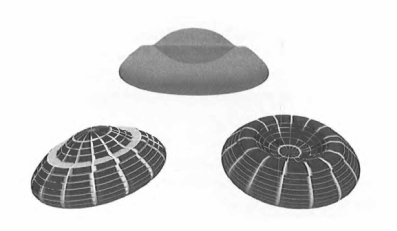
\includegraphics[width=0.8\textwidth]{imagenes/no_rigid}
	\end{center}
	\caption{Superficie no rígida.}
	\label{fig:etiq_2}
\end{figure}




\begin{definicion}
	Diremos que $S \subset \mathbb{R}^3$ es una \underline{\textbf{superficie}} si para todo $p \in S$ existe un entorno $V \subset S$ de $p$, un abierto $U \subset \mathbb{R}^2$ y una aplicación $X : U \to \mathbb{R}^3$ diferenciable tales que:
	\begin{enumerate}
		\item $X(U) = V$,
		\item la aplicación $X : U \to V$ es un homeomorfismo,
		\item $\forall q \in U$, $(dX)_q : \mathbb{R}^2 \to \mathbb{R}^3$ es inyectiva.
	\end{enumerate}
\end{definicion}
${ }$\\

\begin{teorema}
	$\textbf{(Fórmula del cambio de variable)}$ Sea $F : R_1 \to R_2$ un difeomorfismo, siendo $R_1$, $R_2$ de dos superficies orientables, y sea $\Phi : R_2 \to \mathbb{R}$ una función integrable. Entonces, $(\Phi \circ F)(p)|Jac \Phi|(p)$ es integrable y
	\[
	\int_{R_2} \Phi = \int_{R_1} (\Phi \circ F)|Jac \Phi|.
	\]
\end{teorema}
${ }$\\

\begin{teorema}\label{teo:divergencia}
	$\textbf{(Teorema de la divergencia sobre superficies)}$ Sea una superficie compacta $S$ y un campo diferenciable de vectores $V : S \to \mathbb{R}^3$. Entonces:
	\begin{enumerate}
		\item $\int_S div V = -2 \int_S \langle V, N \rangle H$,
		\item $\int_S [k_2(p) \langle (dV)_p(e_1), e_1\rangle + k_1(p) \langle (dV)_p(e_2), e_2 \rangle ] \; dp = -2 \int_S \langle V, N \rangle K$, donde $\{ e_1, e_2 \}$
	\end{enumerate}
\end{teorema}
${ }$\\

\begin{teorema} \label{teo:hadamard}
	$\textbf{(Hadamard-Stoker)}$ Sea un ovaloide $S \subset \mathbb{R}^3$ y $\Omega$ su dominio interior. Entonces:
	
	\begin{enumerate}
		\item Para todo $x, y \in \overline{\Omega}$, entonces $]x, y[ \subset \Omega$. En particular, $\Omega$ es convexo.
		\item Para cada $p \in S$, $\Pi_p \cap S = \{p\}$, donde $\Pi_p$ es el plano tangente afín a $S$ en p. Además, $\overline{\Omega} \subset \bigcap_{p \in S} \; \Pi^{+}_{p}$.
	\end{enumerate}
\end{teorema}
${ }$\\

\begin{teorema}
	$\textbf{(Fórmulas de Minkowski)}$ Sea $S$ una superficie compacta, $N$ su normal interior y $K$, $H$ sus curvaturas de Gauss y media. Entonces, se cumplen las siguientes fórmulas:
	\begin{enumerate}
		\item $\int_S (1 + \langle p, N(p) \rangle H(p) \; dp = 0$,
		\item $\int_S (H(p) + \langle p, N(p) \rangle K(p) \; dp = 0$
	\end{enumerate}
\end{teorema}
${ }$\\

(HACER UN RESPASO DE TODO LO QUE HE HECHO PARA VER QUE METO EN ESTA SECCION)


${ }$\\
${ }$\\
${ }$\\
$\textbf{RAY-MARCHING EVOLUCIÓN}$
${ }$\\

Ray-marching es una tecnica para la visualización de superficies mas complejas dadas en ecuaciones de implicitas que son las de la siguiente forma:

\[
F(x,y,z) = 0.
\]

Esta algoritmo usa el método de newton-raphson para aproximar las soluciones de una función para ir aproximandose iterativamente a la superficie. Comienza en el principio del rayo y avanza a lo largo de él la misma cantidad que la distancia de la superficie al último punto tomado.